\chapter{Phase de développement~: implémentation d'un module statistique}
	\paragraph{}
	Nous avons maintenant une idée précise de ce a quoi devra ressembler le module
	statistiques, il nous faut à présent le développer.
	
	\subsection{Une gestion de projet en mode agile}
		\paragraph{}
		Introduction de la sous partie.
		
		\subsubsection{Une méthodologie qui s'inspire des méthodes agiles}
			\paragraph{}
			
			\begin{figure}[h]% Méthodo de la conception
				\centering
				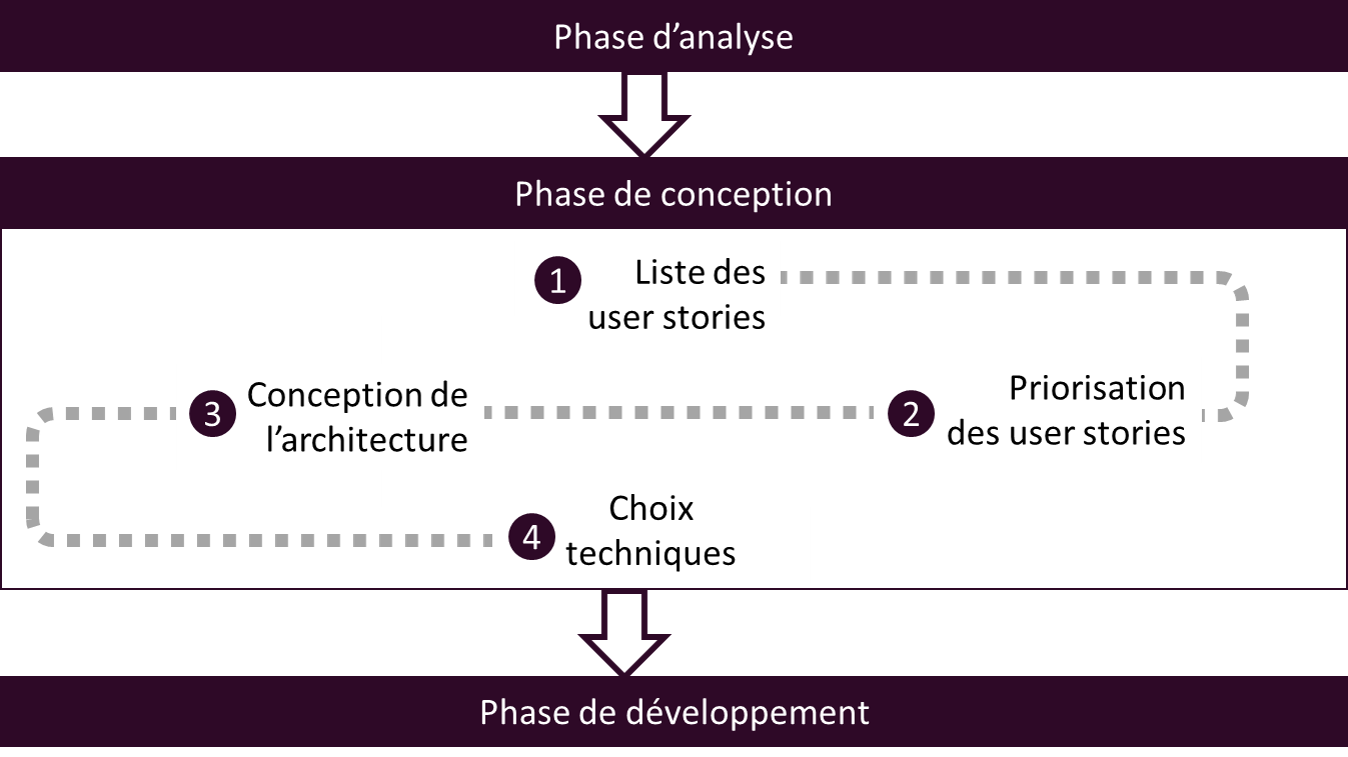
\includegraphics[width=15cm]{../img/part3/methodo_conception.png}
				\caption{\label{methodo_conception} Méthodologie de la conception du
				nouveau module.}
			\end{figure}
			
			\begin{figure}[h]% Méthodo du dééveloppement
				\centering
				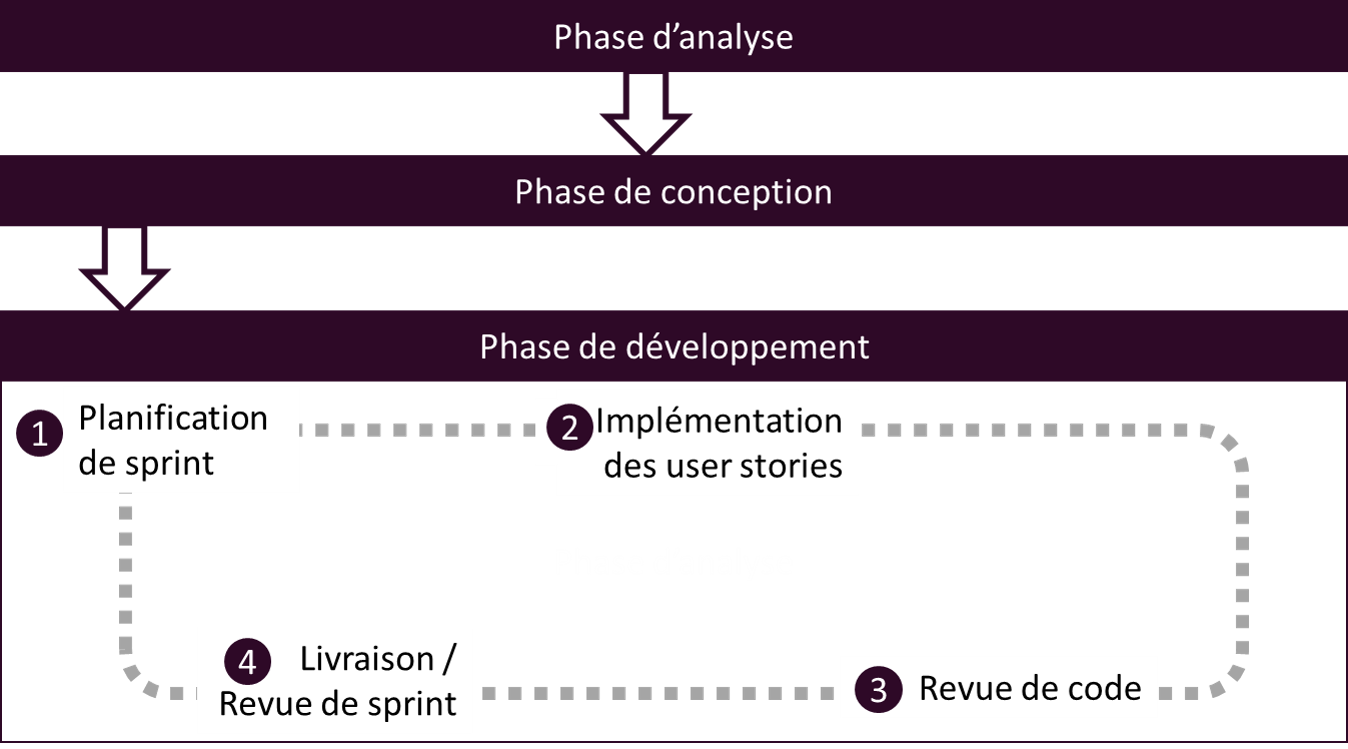
\includegraphics[width=15cm]{../img/part3/methodo_dev.png}
				\caption{\label{methodo_dev} Le développement se déroule en sprints de
				deux semaines chacun.}
			\end{figure}
		
		\subsubsection{Élaboration du backlog}
	
	\subsection{TrackCIS, une application web en deux parties}
		\paragraph{}
		Introduction de la sous partie.
		
		\subsubsection{Qu'est-ce qu'une application web ?}
			\paragraph{}% Modèle client serveur classique
			
			\paragraph{}% Modèle AJAX
			
		\subsubsection{TrackCIS est composé d'un frontal et d'une API}
			\paragraph{}% Archi générale de l'application
			
			%\begin{figure}[h]% Architecture globale de l'application
			%	\centering
			%	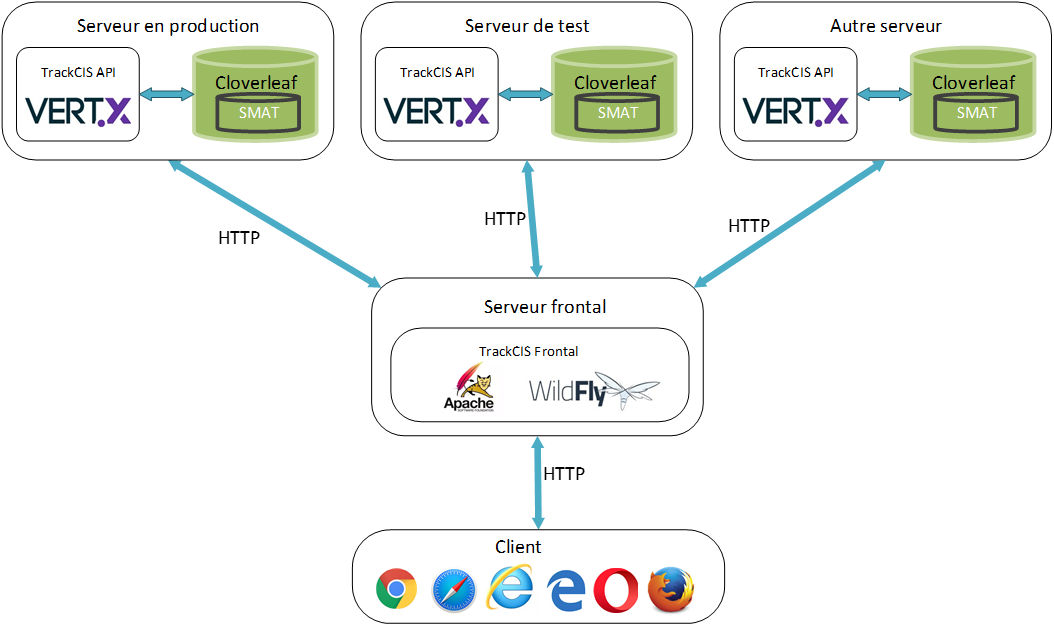
\includegraphics[width=10cm]{../img/part3/archi_trackcis.png}
			%	\caption{\label{archi_trackcis} TrackCIS est composés de deux éléments
			%	distincts pouvant se trouver sur des serveurs différents.}
			%\end{figure}
			
		\subsubsection{Le frontal est développé en java J2EE}
			\paragraph{}% Les bases de la POO
			
			\paragraph{}% les grandes lignes de l'archi du front
			
		\subsubsection{L'API permet de communiquer avec Cloverleaf}
			\paragraph{}% Les grandes lignes de l'archi de l'API
	
	\subsection{L'analyse technique permet l'implémentation du nouveau module à l'existant}
		\paragraph{}
		Introduction de la sous partie.
		
		\subsubsection{Un module qui est basé sur les données disponibles dans
		Cloverleaf}
		\subsubsection{Nouvelle architecture de l'application}
			
		\subsubsection{Réalisation des choix techniques}
			\paragraph{}% Liste des choix
			Le développement de ce projet implique l'utilisation d'un certain nombre de
			technologies. Certaines d'entre elles n'ont pas été utilisée pour le
			développement de la première version de TrackCIS.
			Le tableau ci-dessous résume l'ensemble des technologies qui ont été
			utilisées pour le développement de TrackCIS jusqu'a présent (c'est-à-dire
			avant le présent travail).
			
			\paragraph{}% Méthodo des choix
			Nous n'allons pas ici détaillé tous les choix techniques qui ont été fait.
			Nous mettrons en avant dans cette partie la méthodologie avec laquelle ces
			différents choix tecnique on été effectué en l'illustrant d'un exemple, en
			l'occurence le choix de la bibliothèque graphique javascript.
	
	\subsection{Bilan de la phase de développement et suite du projet}
		\paragraph{}
		Introduction de la sous partie.
		
		\subsubsection{Les fonctionnalités implémentées}
		\subsubsection{Un module maintenable}
			\paragraph{}% Principes et intérêts de la documentation~: plusieurs niveaux
			%  de doc
			\paragraph{}% documentation du code~: la java doc
			\paragraph{}% documentation utilisateur
		\subsubsection{Les suites possibles du projet pour Xperis}
		
		
		
		
		